\documentclass[a4paper, 12pt]{article}%тип документа

%отступы
\usepackage[left=2cm,right=2cm,top=2cm,bottom=3cm,bindingoffset=0cm]{geometry}
\setlength{\parindent}{5ex}

%Русский язык
\usepackage[T2A]{fontenc} %кодировка
\usepackage[utf8]{inputenc} %кодировка исходного кода
\usepackage[english,russian]{babel} %локализация и переносы

%Вставка картинок
\usepackage{graphicx}
\graphicspath{{pictures/}}
\DeclareGraphicsExtensions{.pdf,.png,.jpg}

%Графики
\usepackage{pgfplots}
\pgfplotsset{compat=1.9}

%Математика
\usepackage{amsmath, amsfonts, amssymb, amsthm, mathtools}

%Таблицы
\usepackage{longtable} 
\usepackage{float}

%Римские цифры
\newcommand{\RomanNumeralCaps}[1]{\uppercase\expandafter{\romannumeral#1}}

\usepackage{multirow}

\usepackage{hhline}

\begin{document}
	\begin{titlepage}
		\begin{center}
			\textsc{Федеральное государственное автономное образовательное учреждение высшего образования«Московский физико-технический институт (национальный исследовательский университет)»\\[5mm]
			}
			
			\vfill
			
			\textbf{Вопрос по выбору: \\[3mm]
				Опыт Милликена.
				\\[50mm]
			}
			
		\end{center}
		
		\hfill
		\begin{minipage}{.5\textwidth}
			Выполнил студент:\\[2mm]
			Сериков Василий Романович\\[2mm]
			Группа: Б03-102\\[5mm]
			
		\end{minipage}
		\vfill
		\begin{center}
			Москва, 2022 г.
		\end{center}
		
	\end{titlepage}
	
	\newpage
	\textbf{Аннотация}\\
	
	
	\textbf{Цель работы: }\\
	Измерение элементарного заряда методом масляных капель.\\
	
	\textbf{В работе используется: }\\
	Плоский конденсатор в защитном кожухе, осветитель, измерительный микроскоп, электростатический вольтметр, секундомер, переключатель напряжения, пульверизатор с маслом.\\
	
	\textbf{Теоретические сведения: }\\
	Если элементарный заряд существует, то все заряды будут ему кратны. В опыте будут измерятся заряды капелек масла, несущих несколько элементарных зарядов.\\
	Для измерения заряда будем исследовать движение капелек в электрическом поле. Уравнение движения капли при свободном падении
	\begin{equation}
		m \dfrac{dv}{dt}=mg-F_{\text{тр}},
	\end{equation}
	где $m$ -- масса капли, $v$ -- её скорость, $F_{\text{тр}}=6\pi \eta rv = kv$ -- сила вязкого трения, $r$ -- радиус капли, $\eta$ -- коэффициент вязкости воздуха. Отсюда получаем 
	\begin{equation}
		v = \dfrac{mg}{k}\left(1 - e^{-kt/m}\right).
	\end{equation}
	Скорость установится на
	$$
	v_{\text{уст}}=\dfrac{mg}{k}=\dfrac{2}{9}\dfrac{\rho}{\eta}gr^2,
	$$
	где $\rho$ -- плотность масла. Установление этой скорости происходит с постоянной
	$$
	\tau = \dfrac{m}{k}=\dfrac{2}{9}\dfrac{\rho}{\eta}r^2
	$$
	Обозначая $h$ путь капли, пройденный за $t_0$, получаем формулу для её радуса:
	\begin{equation}
		r = \sqrt{\dfrac{9\eta h}{2\rho gt_0}}.
	\end{equation}
	В случае движения в электрическом поле конденсатора с разностью потенциалов $V$ и расстоянием $l$ между пластинами получаем уравнение движения
	\begin{equation}
		m \dfrac{dv}{dt}=\dfrac{qV}{l}-mg-kv,
	\end{equation}
	Новое слагаемое не влияет на $\tau$, новая установившаяся скорость
	$$
	v_{\text{уст}}'=\dfrac{qV/l - mg}{k}.
	$$
	Если $t$ -- время подъёма на высоту $h$, то можно получить формулу заряда капли:
	$$
	\dfrac{h}{t} = v_{\text{уст}}' = \dfrac{qV}{kl}-v_{\text{уст}};
	$$
	$$
	k=6\pi \eta r  = 6\pi \eta  \sqrt{\dfrac{9\eta h}{2\rho gt_0}};
	$$
	\begin{center}
		$\Rightarrow$ \fbox{$q = 9\pi \sqrt{\dfrac{2\eta^3 h^3}{g\rho}}\cdot \dfrac{l(t_0+t)}{Vt^{3/2}_0t}$}
	\end{center}
	\textbf{Экспериментальная установка: }\\

	Схема установки представлена на рисунке 1. Масло разбрызгивается пульверизатором, попадает на конденсатор $C$ через небольшое отверстие, приобретая заряд из-за трения о воздух.\\
	Напряжение подаётся с выпрямителя и измеряется вольтметром $V$. Ключ $K$ позволяет менять направление поля конденсатора. При замыкании конденсатор разряжается в $R \approx 10~\text{МОм}$.\\
	Для наблюдения за каплями установлен микроскоп, в фокальной плоскости окуляра которого  виден ряд горизонтальных линий с предварительно определенным расстоянием между ними. Время движения капель измеряется электронным секундомером.
	
	\begin{figure}[H]
		\center{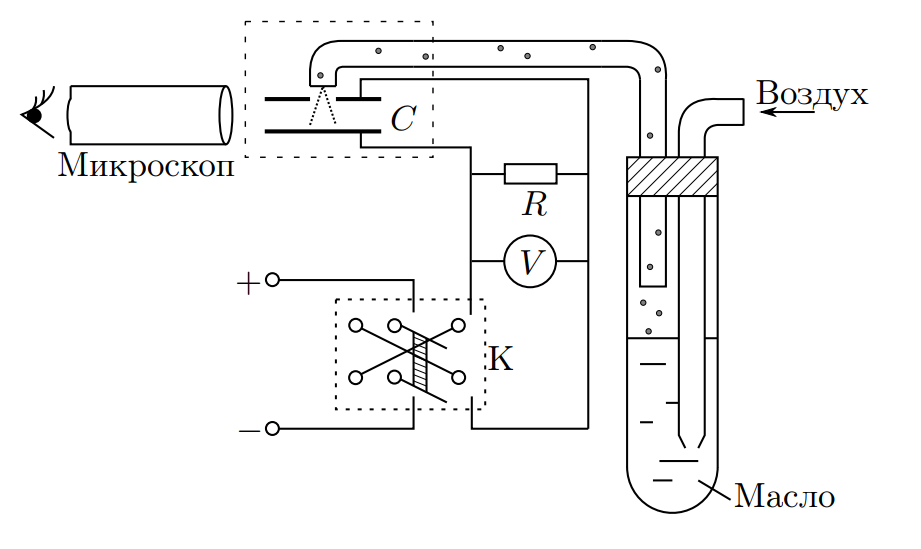
\includegraphics[scale=0.6]{ust.png}}
	\end{figure}


	\textbf{Результаты измерений и обработка данных: }\\
	\begin{enumerate}
	\item Запишем начальные данные и погрешности.\\
	$ h = 1$ мм - расстояние, которое проходит капля в эксперименте.\\
	$ \rho = 898 $ кг/м$^3$ - плотность масла. \\
	$ \eta = 1,83 \cdot 10^{-5}$ Па$\cdot$с - коэффициент трения воздуха.\\ 
	$ l = 0,725$ см - расстояние между пластинами конденсатора.\\
	$\sigma_t = 0,3$ с - погрешность измерения времени.\\
	$ \sigma_v = 20 $ В - погрешность измерения напряжения.\\
	
	\item Проведем серию экспериментов по определению времени $t_0$ и $t_1$ прохождения расстояния h каплей масла под действием силы тяжести $mg$ и под действием электрической силы $qE$. По полученным данным определим заряд капель и занесем все результаты в таблицы 1-5.
	
	\newpage


\begin{longtable} {|c|c|c|c|c|c|c|c|}
	\hline
	\multicolumn{4}{|c|}{№ 1} & \multicolumn{4}{c|}{№ 2} \\ \hline
	$t_0$, c& $t_1$, c & $q$, $\cdot 10^{-19}$ Кл & $\overline{q}$, $\cdot 10^{-19}$ Кл & 	$t_0$, & $t_1$ & $q$, $\cdot 10^{-19}$ Кл & $\overline{q}$, $\cdot 10^{-19}$ Кл\\ \hline
	63,8 & 6,2 & 3,39 & \multirow{5}{*}{3,31} & 58,2 & 7,3 & 3,09 & \multirow{5}{*}{3,13}  \\ \hhline{---~---~}
	62,9 & 6,5 & 3,27 &  & 57,8 & 7,2 & 3,14 &  \\ \hhline{---~---~}
	64,1 & 6,5 & 3,24 &  & 58,4 & 7,2 & 3,12 &  \\ \hhline{---~---~}
	63,3 & 6,3 & 3,36 &  & 59,1 & 7,1 & 3,14 &  \\ \hhline{---~---~}
	63,3 & 6,4 & 3,31 &  & 58,9 & 7,1 & 3,15 &  \\ \hline
\end{longtable}
\begin{longtable} {|c|c|c|c|c|c|c|c|}
	\hline
	\multicolumn{4}{|c|}{№ 3} & \multicolumn{4}{c|}{№ 4} \\ \hline
	$t_0$, c& $t_1$, c & $q$, $\cdot 10^{-19}$ Кл & $\overline{q}$, $\cdot 10^{-19}$ Кл & 	$t_0$, & $t_1$ & $q$, $\cdot 10^{-19}$ Кл & $\overline{q}$, $\cdot 10^{-19}$ Кл\\ \hline
	69,3 & 11,8 & 1,82 & \multirow{5}{*}{1,80} & 51,2 & 4,8 & 4,81 & \multirow{5}{*}{4,90} \\ \hhline{---~---~}
	68,8 & 11,6 & 1,86 &  & 52,3 & 4,9 & 4,72 &  \\ \hhline{---~---~}
	68,9 & 11,9 & 1,82 &  & 51,8 & 4,7 & 4,93 &  \\ \hhline{---~---~}
	71,2 & 12,1 & 1,75 &  & 51,5 & 4,7 & 4,95 &  \\ \hhline{---~---~}
	70,4 & 12,3 & 1,73 &  & 51,4 & 4,6 & 5,05 &  \\ \hline
\end{longtable}
\begin{longtable} {|c|c|c|c|c|c|c|c|}
	\hline
	\multicolumn{4}{|c|}{№ 5} & \multicolumn{4}{c|}{№ 6} \\ \hline
	$t_0$, c& $t_1$, c & $q$, $\cdot 10^{-19}$ Кл & $\overline{q}$, $\cdot 10^{-19}$ Кл & 	$t_0$, & $t_1$ & $q$, $\cdot 10^{-19}$ Кл & $\overline{q}$, $\cdot 10^{-19}$ Кл\\ \hline
	52,3 & 8,0 & 3,05 & \multirow{5}{*}{3,10} & 61,2 & 13,5 & 1,77 & \multirow{5}{*}{1,75} \\ \hhline{---~---~}
	51,9 & 7,9 & 3,10 &  & 61,4 & 13,7 & 1,74 &  \\ \hhline{---~---~}
	51,7 & 8,0 & 3,07 &  & 61,5 & 13,7 & 1,74 &  \\ \hhline{---~---~}
	51,4 & 7,8 & 3,15 &  & 61,8 & 13,5 & 1,76 &  \\ \hhline{---~---~}
	51,5 & 7,8 & 3,15 &  & 62,0 & 13,6 & 1,74 &  \\ \hline
\end{longtable}
\begin{longtable} {|c|c|c|c|c|c|c|c|}
	\hline
	\multicolumn{4}{|c|}{№ 7} & \multicolumn{4}{c|}{№ 8} \\ \hline
	$t_0$, c& $t_1$, c & $q$, $\cdot 10^{-19}$ Кл & $\overline{q}$, $\cdot 10^{-19}$ Кл & 	$t_0$, & $t_1$ & $q$, $\cdot 10^{-19}$ Кл & $\overline{q}$, $\cdot 10^{-19}$ Кл\\ \hline
	50,1 & 4,3 & 5,46 & \multirow{5}{*}{5,41} & 53,5 & 7,5 & 3,18 & \multirow{5}{*}{3,17} \\ \hhline{---~---~}
	50,8 & 4,2 & 5,53 &  & 53,6 & 7,4 & 3,21 &  \\ \hhline{---~---~}
	50,7 & 4,4 & 5,31 &  & 53,8 & 7,5 & 3,17 &  \\ \hhline{---~---~}
	50,9 & 4,4 & 5,30 &  & 53,7 & 7,6 & 3,14 &  \\ \hhline{---~---~}
	50,5 & 4,3 & 5,43 &  & 54,0 & 7,6 & 3,13 &  \\ \hline
\end{longtable}
\begin{longtable} {|c|c|c|c|c|c|c|c|}
	\hline
	\multicolumn{4}{|c|}{№ 9} & \multicolumn{4}{c|}{№ 10} \\ \hline
	$t_0$, c& $t_1$, c & $q$, $\cdot 10^{-19}$ Кл & $\overline{q}$, $\cdot 10^{-19}$ Кл & 	$t_0$, & $t_1$ & $q$, $\cdot 10^{-19}$ Кл & $\overline{q}$, $\cdot 10^{-19}$ Кл\\ \hline
	51,1 & 14,4 & 1,9 & \multirow{5}{*}{1,85} & 58,9 & 7,3 & 3,07 & \multirow{5}{*}{3,12} \\ \hhline{---~---~}
	51,8 & 14,8 & 1,85 &  & 58,0 & 7,2 & 3,14 &  \\ \hhline{---~---~}
	51,5 & 14,7 & 1,86 &  & 58,4 & 7,2 & 3,12 &  \\ \hhline{---~---~}
	51,4 & 14,9 & 1,83 &  & 59,1 & 7,1 & 3,14 &  \\ \hhline{---~---~}
	51,9 & 14,8 & 1,84 &  & 58,9 & 7,1 & 3,15 &  \\ \hline
\end{longtable}
\center{Таблицы 1-5: Полученные данные для времени и расчет значения заряда капель. }
	
	
	
	
	
	
	
	
	
	
	
	
	
	
	
	
	
	
	
	
	
	
	
	
	
	
	
	\end{enumerate}
	
	
	
	\end{document}